% Lecture Template for ME3023 -  Measurements in Mechanical Systems - Tennessee Technological University
% Spring 2020 - Summer 2020 - Fall 2020 - Spring 2021 - Summer 2021 - Fall 2023
% Tristan Hill, May 07, 2020 - June 12, 2020 - July 08, 2020 - Novemeber 02, 2020 - March 28, 2021 - May 25, 2021 - August 21, 2022 - September 02, 2023 - September 09, 2023 - April 07, 2024 - November 18, 2024

% Fall 2023 - condensing and streamlining lectures by combining topics into a single PDF under the module name
%			  this will simplify file and link management as well as make lectures easier to use in class
%			- added image/ to clean directory and reduce redundancy, specific to module for now  

% Module Name: - Strain Applications

\documentclass[fleqn]{beamer} % for presentation (has nav buttons at bottom)
\usepackage{../measurements_lectures}

\author{ME3023 - Measurements in Mechanical Systems} 

\newcommand{\MNUM}{9\hspace{2mm}} % module number 
\newcommand{\moduletitle}{Strain Applications}

\newcommand{\sectionItitle}{Beam Models}
\newcommand{\sectionIItitle}{}
\newcommand{\sectionIIItitle}{}

\newcommand{\sectionIsubsectionItitle}{Euler–Bernoulli Beam Theory}
\newcommand{\sectionIsubsectionIItitle}{Force-Deflection Model}
\newcommand{\sectionIsubsectionIIItitle}{Cantilevered Beam}
\newcommand{\sectionIsubsectionIVtitle}{Deflection and Strain}

\newcommand{\sectionIIsubsectionItitle}{}
\newcommand{\sectionIIsubsectionIItitle}{}
\newcommand{\sectionIIsubsectionIIItitle}{}
\newcommand{\sectionIIsubsectionIVtitle}{}

\newcommand{\sectionIIIsubsectionItitle}{}
\newcommand{\sectionIIIsubsectionIItitle}{}
\newcommand{\sectionIIIsubsectionIIItitle}{}
\newcommand{\sectionIIIsubsectionIVtitle}{}

 \newcommand{\btVFill}{\vskip0pt plus 1filll}

% custom box
\newsavebox{\mybox}

\title{Lecture Module - \moduletitle}

\date{Mechanical Engineering\vspc Tennessee Technological University}

\begin{document}

	\lstset{language=MATLAB,basicstyle=\ttfamily\small,showstringspaces=false}

	\frame{\titlepage \center\begin{framed}\Large \textbf{Module \MNUM - \moduletitle}\end{framed} \vspace{5mm}}

	% Module Outline
	\begin{frame} 
		\large \textbf{Module \MNUM - \moduletitle} \vspace{3mm}\\

		\begin{itemize}
			\item Topic 1 - \hyperlink{sectionI}{\sectionItitle} \vspc % section I
			\item Topic 2 - \hyperlink{sectionII}{\sectionIItitle} \vspc % section II
			\item Topic 3 - \hyperlink{sectionIII}{\sectionIIItitle} \vspc % section III
		\end{itemize}

	\end{frame}

	% section I
	\section{\sectionItitle}\label{sectionI}

		% section I Outline
		\begin{frame} 
			\large \textbf{Topic 1 - \sectionItitle} \vspace{3mm}\\

			\begin{multicols}{2}
			\begin{itemize}
				\item \hyperlink{sectionIsubsectionI}{\sectionIsubsectionItitle} \vspc %  section I subsection I
				\item \hyperlink{sectionIsubsectionII}{\sectionIsubsectionIItitle} \vspc % section I subsection II
				\item \hyperlink{sectionIsubsectionIII}{\sectionIsubsectionIIItitle} \vspc % section I subsection III
				\item \hyperlink{sectionIsubsectionIV}{\sectionIsubsectionIVtitle} \vspc % section I subsection IV
			\end{itemize}

			\includegraphics[scale=0.28]{images/leonhard_euler.jpg}
			\includegraphics[scale=1.7]{images/daniel_bernoulli.jpg}

			\end{multicols}
		\end{frame}
		
		% section I subsection I 
		\subsection{\sectionIsubsectionItitle}\label{sectionIsubsectionI}

			\begin{frame}
				\frametitle{\sectionIsubsectionItitle}
				\bigskip

				Euler–Bernoulli beam theory (also known as engineer's beam theory or classical beam theory)[1] is a simplification of the linear theory of elasticity which provides a means of calculating the load-carrying and deflection characteristics of beams. It covers the case for small deflections of a beam that are subjected to lateral loads only. 
				\btVFill
				{\tiny Text: \href{https://en.wikipedia.org/wiki/Euler\%E2\%80\%93Bernoulli_beam_theory}{Wikipedia}}

			\end{frame}

			\begin{frame}
				\frametitle{\sectionIsubsectionItitle}
				\bigskip

				It is thus a special case of Timoshenko beam theory. It was first enunciated circa 1750,[2] but was not applied on a large scale until the development of the Eiffel Tower and the Ferris wheel in the late 19th century. Following these successful demonstrations, it quickly became a cornerstone of engineering and an enabler of the Second Industrial Revolution.\vspc

				Additional mathematical models have been developed such as plate theory, but the simplicity of beam theory makes it an important tool in the sciences, especially structural and mechanical engineering. 

				\btVFill
				{\tiny Text: \href{https://en.wikipedia.org/wiki/Euler\%E2\%80\%93Bernoulli_beam_theory}{Wikipedia}}

				
			
			\end{frame}


		% section I subsection II
		\subsection{\sectionIsubsectionIItitle}\label{sectionIsubsectionII}

			\begin{frame}
				\frametitle{\sectionIsubsectionIItitle}\small
				\bigskip

				\begin{multicols}{2}
					\includegraphics[scale=.4]{images/diving_board_cut.png}
					\small
					These stiffness equations come from the beam deflection equations you have and will study.\vspc 
					You can see them \href{https://mechanicalc.com/reference/beam-deflection-tables}{{\BL here}} or look in your copy of Shigleys, and here is a good section on beam analysis \href{https://mechanicalc.com/reference/beam-analysis}{\BL analysis}.


					\includegraphics[scale=.2]{images/types_of_springs.png}
				\end{multicols}
							
				\btVFill
				
			\end{frame}

			\begin{frame}
				\frametitle{\sectionIsubsectionIItitle}\small
				\bigskip


				\btVFill
				

			\end{frame}

		% section I subsection III
		\subsection{\sectionIsubsectionIIItitle}\label{sectionIsubsectionIII}
			\begin{frame} 
				\frametitle{\sectionIsubsectionIIItitle} %\scriptsize


				The beam equations relate internal moment and shear as well as deflection along the length of the beam to the given beam geometry and loading.  

				\begin{multicols}{2}

				\includegraphics[scale=.50]{images/cantelever_deflection.png}

				\vspace{10mm}
				\hspccc\scalebox{1}{$\delta(x)=-\frac{Fx^2}{6EI}(3L-x)$} \vspc
				\hspccc\scalebox{1}{$\delta_{max}=\delta|_{x=L}=-\frac{FL^3}{3EI}$} \vspccc
				\hspccc\scalebox{1}{$\theta(x)=-\frac{Fx}{2EI}(2L-x)$} \vspc
				\hspccc\scalebox{1}{$\theta_{max}=\theta|_{x=L}=-\frac{FL^2}{2EI}$}

				\end{multicols}

				\bigskip

			\end{frame}	

			\begin{frame} 
				\frametitle{\sectionIsubsectionIIItitle}
				The shear and moment are both given as a function of x, the direction along the beam. 

				\begin{multicols}{2}

				\includegraphics[scale=.5]{images/cantelever_beam.png}

				\scalebox{1}{$M(x)=-F(L-x)$}\vspcc
				\scalebox{1}{$M_{max}=M|_{x=0}=-FL$}

				\end{multicols}
			
				\bigskip
							
			\end{frame}	

			\begin{frame} 
				\frametitle{\sectionIsubsectionIIItitle}
				The internal stress is given as a function of y, the distance from the neutral axis. \vspccc

				\begin{multicols}{2}

				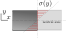
\includegraphics[scale=.75]{images/internal_stress.png}

				\scalebox{1}{$\sigma=\frac{Mc}{I}$}\vspc

				\end{multicols}

				\vspace{20mm}
				{\tiny Text: Theory and Design of Mechanical Measurements}
							
				\bigskip
			

				
			\end{frame}	

		% section I subsection IV
		\subsection{\sectionIsubsectionIVtitle}\label{sectionIsubsectionIV}	

			\begin{frame}
				\frametitle{\sectionIsubsectionIVtitle} \scriptsize
				\bigskip

				Now, with the beam equations you can relate measured strain at a known location to deflection at the end of the beam.These equations are available for many different beam types and loading conditions. {\tiny \href{https://mechanicalc.com/reference/beam-deflection-tables}{{\BL Beam Eq's}}}  \vspc

				\includegraphics[scale=.4]{images/axial_gaged_beam.png}

			
				\btVFill
			

			\end{frame}

			\begin{frame}
				\frametitle{\sectionIsubsectionIVtitle} \scriptsize


			\end{frame}


			\begin{frame}
				\frametitle{\sectionIsubsectionIVtitle} \scriptsize

				\bigskip


				\btVFill

										
			\end{frame}

	
	% Section II
	\section{\sectionIItitle}\label{sectionII}

		% section II Outline
		\begin{frame}
			\large \textbf{Topic 2 - \sectionIItitle} \vspace{3mm}\\

			\begin{itemize}
				\item \hyperlink{sectionIIsubsectionI}{\sectionIIsubsectionItitle} \vspc %  section II subsection I
				\item \hyperlink{sectionIIsubsectionII}{\sectionIIsubsectionIItitle} \vspc % section II subsection II
				\item \hyperlink{sectionIIsubsectionIII}{\sectionIIsubsectionIIItitle} \vspc % section II subsection III
				\item \hyperlink{sectionIIsubsectionIV}{\sectionIIsubsectionIVtitle} \vspc % section II subsection IV
			\end{itemize}

		\end{frame}

		% section II subsection I
		\subsection{\sectionIIsubsectionItitle}\label{sectionIIsubsectionI}

			\begin{frame}[label=sectionIIsubsectionI]
				\frametitle{\sectionIIsubsectionItitle} \scriptsize

				\bigskip	
				
				\btVFill
				
		
			\end{frame}

		    \begin{frame}[label=sectionIIsubsectionI]
				\frametitle{\sectionIIsubsectionItitle} \scriptsize

				
				\btVFill

			
					
			\end{frame}	


		% section II subsection II
		\subsection{\sectionIIsubsectionIItitle}\label{sectionIIsubsectionII}

			\begin{frame}
				\frametitle{\sectionIIsubsectionIItitle} \scriptsize
				\bigskip

				
				\btVFill
				

			\end{frame}

			\begin{frame}
				\frametitle{\sectionIIsubsectionIItitle} \scriptsize
	
				\bigskip

				
				\btVFill
			
				
			\end{frame}

		% section II subsection III
		\subsection{\sectionIIsubsectionIIItitle}\label{sectionIIsubsectionIII}

			\begin{frame}
				\frametitle{\sectionIIsubsectionIIItitle} 

				\bigskip

				
				\btVFill
				

			\end{frame}

			\begin{frame}
				\frametitle{\sectionIIsubsectionIIItitle}

				\bigskip


				\btVFill
			
			\end{frame}

			\begin{frame}
			\frametitle{\sectionIIsubsectionIIItitle}




				\btVFill

			\end{frame}

		% section II subsection IV 
		\subsection{\sectionIIsubsectionIVtitle}\label{sectionIIsubsectionIV}

			\begin{frame}
				\frametitle{\sectionIIsubsectionIVtitle}

			\end{frame}

			\begin{frame}
				\frametitle{\sectionIIsubsectionIVtitle}


			\end{frame}
		
	% Section III
	\section{\sectionIIItitle}\label{sectionIII}

		% section III Outline
		\begin{frame}
			\large \textbf{Topic 3 - \sectionIIItitle} \vspace{3mm}\\

			\begin{itemize}
				\item \hyperlink{sectionIIIsubsectionI}{\sectionIIIsubsectionItitle} \vspc %  section III subsection I
				\item \hyperlink{sectionIIIsubsectionII}{\sectionIIIsubsectionIItitle} \vspc % section III subsection II
				\item \hyperlink{sectionIIIsubsectionIII}{\sectionIIIsubsectionIIItitle} \vspc % section III subsection III
				\item \hyperlink{sectionIIIsubsectionIV}{\sectionIIIsubsectionIVtitle} \vspc % section III subsection IV
			\end{itemize}

		\end{frame}

		% section III subsection I
		\subsection{\sectionIIIsubsectionItitle}\label{sectionIIIsubsectionI}

			\begin{frame}
				\frametitle{\sectionIIIsubsectionItitle}

				\bigskip

				
			
				\btVFill
			

			\end{frame}

			\begin{frame}
				\frametitle{\sectionIIIsubsectionItitle}
		
			\end{frame}

		% section III subsection II
		\subsection{\sectionIIIsubsectionIItitle}\label{sectionIIIsubsectionII}	

			\begin{frame}
				\frametitle{\sectionIIIsubsectionIItitle}

				\bigskip

				

				\btVFill

			\end{frame}

			\begin{frame}
				\frametitle{\sectionIIIsubsectionIItitle}

				\bigskip
			
			
				\btVFill

			\end{frame}

			\begin{frame}
				\frametitle{\sectionIIIsubsectionIItitle}

				\bigskip

				

				\btVFill
				
			\end{frame}

		% section III subsection III
		\subsection{\sectionIIIsubsectionIIItitle}\label{sectionIIIsubsectionIII}	

			\begin{frame}[containsverbatim]
				\frametitle{\sectionIIIsubsectionIIItitle}\scriptsize
				
						
			
			\end{frame}


			\begin{frame}[containsverbatim]
				\frametitle{\sectionIIIsubsectionIIItitle}\scriptsize

				

				

			\end{frame}

			

		% section III subsection IV
		\subsection{\sectionIIIsubsectionIVtitle}\label{sectionIIIsubsectionIV}	
		
		% section III subsection IV - Frame I
		\begin{frame} \scriptsize
		\frametitle{\sectionIIIsubsectionIVtitle}
		\bigskip




		\btVFill

		\end{frame}
	

\end{document}





